\documentclass[12pt]{article}
\usepackage{amsmath, amssymb, amsthm}
\usepackage{graphicx}
\graphicspath{ {./../images/} }
\usepackage{amscd}
\usepackage{enumerate}
\usepackage{color}
\usepackage{cancel}
\usepackage{tikz}
\usepackage{empheq}
\usetikzlibrary{matrix}
\usepackage[thinlines]{easytable}
\usepackage[left=2cm,top=1.5cm,right=2cm,bottom=1cm,nohead,nofoot]{geometry}

% define an "answer box" for highlighting final answer
\definecolor{anscolor}{rgb}{.87, .77, 1}

\newlength\mytemplen
\newsavebox\mytempbox

\makeatletter
\newcommand\ansbox{%
    \@ifnextchar[%]
       {\@ansbox}%
       {\@ansbox[0pt]}}

\def\@ansbox[#1]{%
    \@ifnextchar[%]
       {\@@ansbox[#1]}%
       {\@@ansbox[#1][0pt]}}

\def\@@ansbox[#1][#2]#3{
    \sbox\mytempbox{#3}%
    \mytemplen\ht\mytempbox
    \advance\mytemplen #1\relax
    \ht\mytempbox\mytemplen
    \mytemplen\dp\mytempbox
    \advance\mytemplen #2\relax
    \dp\mytempbox\mytemplen
    \colorbox{anscolor}{\hspace{1em}\usebox{\mytempbox}\hspace{1em}}}

\makeatother

% DOCUMENT BEGINNING %
\begin{document}

\begin{center}
    Lecture 1: Introduction
\end{center}

%%%%%%%%%%%%%%%
% PROBLEM 1.1 %
%%%%%%%%%%%%%%%
\subsubsection*{P1.1}
We begin by massaging this complex exponential into a different form using Euler's formula for ease of use in the questions that follow
\begin{equation*}
    \frac{1}{2} e^{\frac{j\pi}{4}} = 
    \frac{1}{2} ( cos(\frac{\pi}{4}) + j sin(\frac{\pi}{4}) ) =
    \frac{1}{2} (\frac{\sqrt{2}}{2}) + j \frac{1}{2} (\frac{\sqrt{2}}{2}) = 
    \frac{\sqrt{2}}{4} + j \frac{\sqrt{2}}{4} 
\end{equation*}

\noindent \textbf{(a)} 
\begin{empheq}[box={\ansbox}]{equation*}
    Re\{z\} = \frac{\sqrt{2}}{4}
\end{empheq}
~\\

\noindent \textbf{(b)} 
\begin{empheq}[box={\ansbox}]{equation*}
    Im\{z\} = \frac{\sqrt{2}}{4}
\end{empheq}
~\\

\noindent \textbf{(c)} 
\begin{equation*}
    \vert z \vert = 
    \sqrt{(\frac{\sqrt{2}}{4})^2 + (\frac{\sqrt{2}}{4})^2} = 
    \sqrt{\frac{2}{16} + \frac{2}{16}} = 
    \sqrt{\frac{4}{16}} = 
    \frac{2}{4} = 
    \frac{1}{2}
\end{equation*}
\begin{empheq}[box={\ansbox}]{equation*}
    \vert z \vert = 
    \frac{1}{2}
\end{empheq}

\noindent \emph{As a side note on this problem, any complex exponential without a coefficient ($e^{jx}$ for some $x$) has a magnitude of $1$. Thus, the magnitude simply becomes the leading coefficient, which is $\frac{1}{2}$ in this case.}
~\\

\noindent \textbf{(d)} 
\begin{empheq}[box={\ansbox}]{equation*}
    \measuredangle z = \frac{\pi}{4}
\end{empheq}
~\\

\noindent \textbf{(e)} 
\begin{empheq}[box={\ansbox}]{equation*}
    z^* = \frac{\sqrt{2}}{4} - j \frac{\sqrt{2}}{4}
\end{empheq}
~\\

\noindent \textbf{(f)} 
\begin{equation*}
    z + z^* = 
    (\frac{\sqrt{2}}{4} + j \frac{\sqrt{2}}{4}) + (\frac{\sqrt{2}}{4} - j \frac{\sqrt{2}}{4}) = 
    \frac{\sqrt{2}}{4} + \frac{\sqrt{2}}{4} = 
    \frac{2\sqrt{2}}{4} = 
    \frac{\sqrt{2}}{2}
\end{equation*}
\begin{empheq}[box={\ansbox}]{equation*}
    z + z^* = \frac{\sqrt{2}}{2}
\end{empheq}
~\\

%%%%%%%%%%%%%%%
% PROBLEM 1.2 %
%%%%%%%%%%%%%%%
\newpage
\subsubsection*{P1.2}
\noindent \textbf{(a)} 
\begin{equation*}
    Re\{z\} = 
    \frac{z + z^*}{2} = 
    \frac{(Re\{z\} + jIm\{z\}) + (Re\{z\} - jIm\{z\})}{2} = 
    \frac{2Re\{z\}}{2} = Re\{z\}
\end{equation*}
~\\

\noindent \textbf{(b)}
\begin{equation*}
    jIm\{z\} = 
    \frac{z - z^*}{2} = 
    \frac{(Re\{z\} + jIm\{z\}) - (Re\{z\} - jIm\{z\})}{2} = 
    \frac{2jIm\{z\}}{2} = 
    jIm\{z\}
\end{equation*}
~\\

%%%%%%%%%%%%%%%
% PROBLEM 1.3 %
%%%%%%%%%%%%%%%
\subsubsection*{P1.3}
\noindent \textbf{(a)} According to Euler's formula, $Re\{e^{j \theta}\} = cos (\theta)$. Therefore, by P1.2(a), 
\begin{equation*}
    cos(\theta) = \frac{e^{j \theta} + e^{-j \theta}}{2}
\end{equation*}
For clarity you can also prove this directly like so
\begin{equation*}
    \frac{e^{j \theta} + e^{-j \theta}}{2} = 
    \frac{(cos(\theta) + jsin(\theta)) + (cos(\theta) - jsin(\theta))}{2} = 
    \frac{2cos(\theta)}{2} = 
    cos(\theta)
\end{equation*}

\noindent \textbf{(b)} According to Euler's formula, $Im\{e^{j \theta}\} = sin (\theta)$. Therefore, by P1.2(b), 
\begin{equation*}
    j sin(\theta) = \frac{e^{j \theta} - e^{-j \theta}}{2}
\end{equation*}
\begin{equation*}
    sin(\theta) = \frac{e^{j \theta} - e^{-j \theta}}{j2}
\end{equation*}
For clarity you can also prove this directly like so
\begin{equation*}
    \frac{e^{j \theta} - e^{-j \theta}}{2j} = 
    \frac{(cos(\theta) + jsin(\theta)) - (cos(\theta) - jsin(\theta))}{2j} = 
    \frac{2jsin(\theta)}{2j} = 
    sin(\theta)
\end{equation*}

%%%%%%%%%%%%%%%
% PROBLEM 1.4 %
%%%%%%%%%%%%%%%
\newpage
\subsubsection*{P1.4}
\noindent \textbf{(a)(i)}
\begin{empheq}[box={\ansbox}]{equation*}
    z^* = re^{-j\theta}
\end{empheq}

\noindent \textbf{(a)(ii)}
\begin{equation*}
    z^2 = (re^{j\theta})^2 = r^2 e^{j2\theta}
\end{equation*}
\begin{empheq}[box={\ansbox}]{equation*}
    z^2 = r^2 e^{j2\theta}
\end{empheq}

\noindent \textbf{(a)(iii)}
\begin{equation*}
    jz = jre^{j\theta} = 
    e^{\frac{\pi}{2}}re^{j\theta} = 
    re^{j\theta + \frac{\pi}{2}}
\end{equation*}
\begin{empheq}[box={\ansbox}]{equation*}
    jz = re^{j\theta + \frac{\pi}{2}}
\end{empheq}

\noindent \textbf{(a)(iv)}
\begin{equation*}
    zz^* = re^{j\theta}re^{-j\theta} = 
    r^2e^{j\theta - j\theta} = 
    r^2e^{0} = 
    r^2
\end{equation*}
\begin{empheq}[box={\ansbox}]{equation*}
    zz^* = r^2
\end{empheq}

\noindent \textbf{(a)(v)}
\begin{equation*}
    \frac{z}{z^*} = 
    z\frac{1}{z^*} = 
    re^{j\theta}\frac{1}{re^{-j\theta}} = 
    e^{j\theta}{e^{j\theta}} = 
    e^{j\theta + j\theta} = 
    e^{j2\theta}
\end{equation*}
\begin{empheq}[box={\ansbox}]{equation*}
    zz^* = e^{j2\theta}
\end{empheq}

\noindent \textbf{(a)(vi)}
\begin{equation*}
    \frac{1}{z} = 
    \frac{1}{re^{j\theta}} = 
    \frac{e^{-j\theta}}{r}
\end{equation*}
\begin{empheq}[box={\ansbox}]{equation*}
    \frac{1}{z} = \frac{e^{-j\theta}}{r}
\end{empheq}

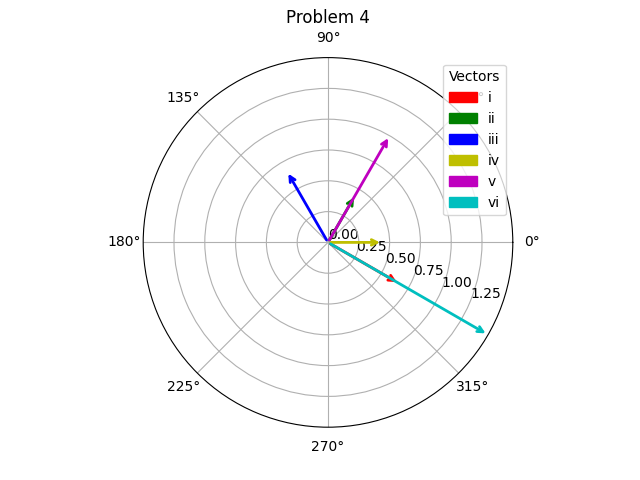
\includegraphics{prob4.png}


%%%%%%%%%%%%%%%
% PROBLEM 1.5 %
%%%%%%%%%%%%%%%
\newpage
\subsubsection*{P1.5}
\begin{equation*}
    2 \sin(\frac{\alpha}{2}) e^{j\frac{\alpha - \pi}{2}} = 
    2 \frac{e^{j\frac{\alpha}{2}} - e^{-j\frac{\alpha}{2}}}{2j} 
    e^{j(\frac{\alpha}{2} - \frac{\pi}{2}}) = 
    \frac{e^{j(\frac{\alpha}{2} + \frac{\alpha}{2} - \frac{\pi}{2}}) - 
    e^{j(\frac{\alpha}{2} - \frac{\alpha}{2} - \frac{\pi}{2}})}{j} = 
    \frac{e^{j(\alpha - \frac{\pi}{2})} - e^{-j\frac{\pi}{2}}}{j}
\end{equation*}
\begin{equation*}
    = \frac{e^{j\alpha} e^{-j\frac{\pi}{2}} - e^{-j\frac{\pi}{2}}}{j} = 
    \frac{e^{-j\frac{\pi}{2}} (e^{j\alpha} - 1)}{j} = 
    \frac{(\cos(\frac{\pi}{2}) -j\sin(\frac{\pi}{2}) (e^{j\alpha} - 1)}{j} = 
    \frac{-j (e^{j\alpha} - 1)}{j} = 
    (1 - e^{j\alpha}) 
\end{equation*}

%%%%%%%%%%%%%%%
% PROBLEM 1.6 %
%%%%%%%%%%%%%%%
\subsubsection*{P1.6}
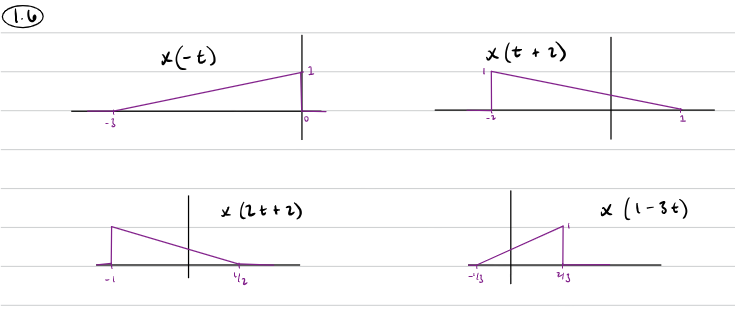
\includegraphics{prob6.png}

%%%%%%%%%%%%%%%
% PROBLEM 1.7 %
%%%%%%%%%%%%%%%
\subsubsection*{P1.7}
\textbf{a)} 
\[ 
\int_{0}^{a} e^{-2t} dt = 
\frac{-1}{2} e^{-2t} \biggr\vert_{0}^{a} = 
\frac{-1}{2} (e^{-2a} - e^{0}) =
\frac{1}{2} (1 - e^{-2a})
\]
\begin{empheq}[box={\ansbox}]{equation*}
    \int_{0}^{a} e^{-2t} dt = \frac{1}{2} (1 - e^{-2a})
\end{empheq}

\textbf{b)} 
\[ 
\int_{2}^{\infty} e^{-3t} dt = 
\frac{-1}{3} e^{-3t} \biggr\vert_{2}^{\infty} = 
\lim_{\tau \to \infty}\frac{-1}{3} (e^{-2\tau} - e^{-3(2)}) =
\frac{e^{-6}}{3}
\]
\begin{empheq}[box={\ansbox}]{equation*}
    \int_{2}^{\infty} e^{-3t} dt = \frac{e^{-6}}{3}
\end{empheq}

\end{document}